% !TEX root = ../rawlik-phd-thesis.tex
\chapter{Next generation active magnetic field compensation}
\label{ch:sfc-prototype}

The coil design method described in the previous chapter opened the door to a next generation of active magnetic field compensation systems. Ones where the coil system is not much larger than the fiducial volume and where high-order terms of the magnetic field can be compensated. All while retaining a low number of controlled degrees of freedom.

The large fiducial volume is of particular importance for the n2EDM experiment at PSI. The available area\ldots

In the laboratory at ETH Zürich an active magnetic field compensation system was constructed, based on the coil design method described earlier. The goal was do demonstrate the feasibility of construction of the coils, develop and test the electronic and software parts of the feedback algorithm, and test the whole system.



\section{The first iteration -- coil structure}
When discussing the the coil design method we have already indicated a possible way to realise it in practice---construct a grid out of cable channels. The system, pictured in Fig.\,\ref{fig:prototype_photo}, was built as a $5 \times 9 \times 5$ square tiles. The tile size\ldots The total size\ldots
\mnote{Introduce the coordinate system somewhere here.}

\begin{figure}
  \centering
  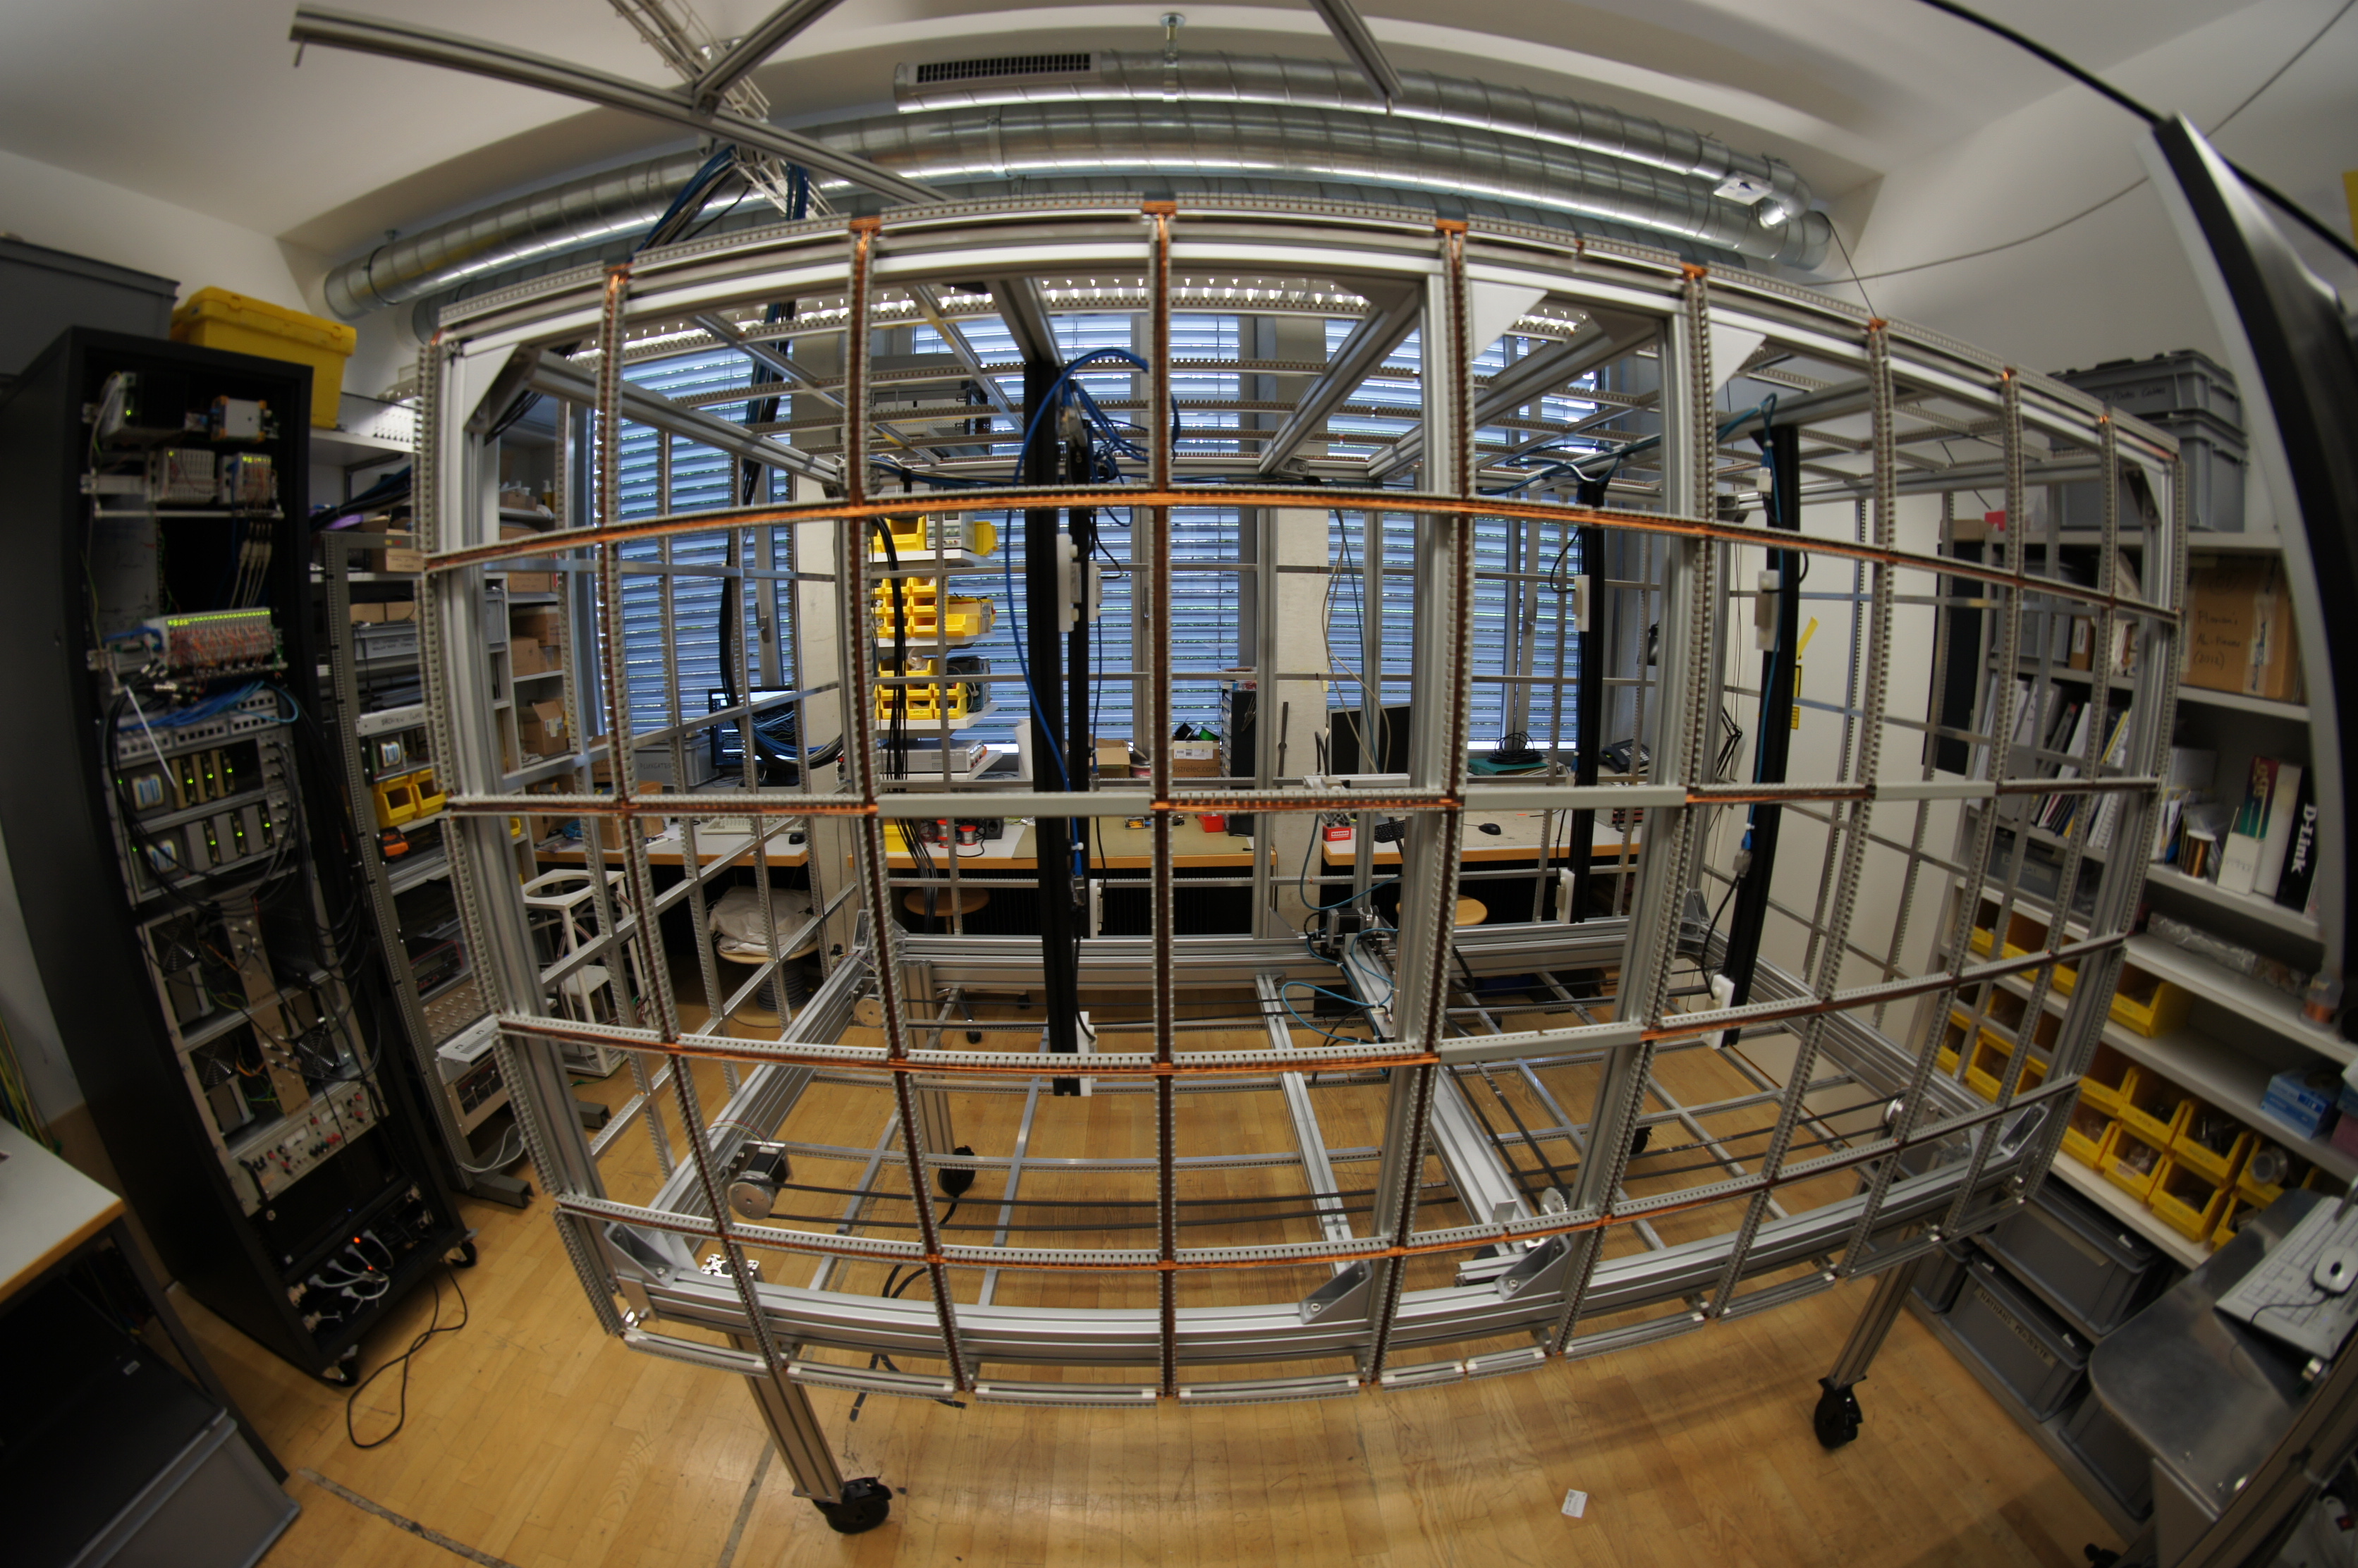
\includegraphics[width=0.9\linewidth]{gfx/prototype/DSC03472.JPG}
  \caption{The active magnetic compensation system in the laboratory at ETH Zürich. It consists cable channels mounted on an aluminum support structure. In the channels copper wires making up the coils can be seen. On the left-hand side the control cabinet of the system is visible. Indicate the coordinate system here!}
  \label{fig:prototype_photo}
\end{figure}

The support frame was made of aluminum construction profiles. Thereon, on each side, was a large one-piece aluminum sheet, with square cut-outs leaving the material only directly below the cable channels. \note{Explain better, tricky.}

and a close-up in \note{put a photo of a close-up, too}.

\begin{figure}
  \centering
  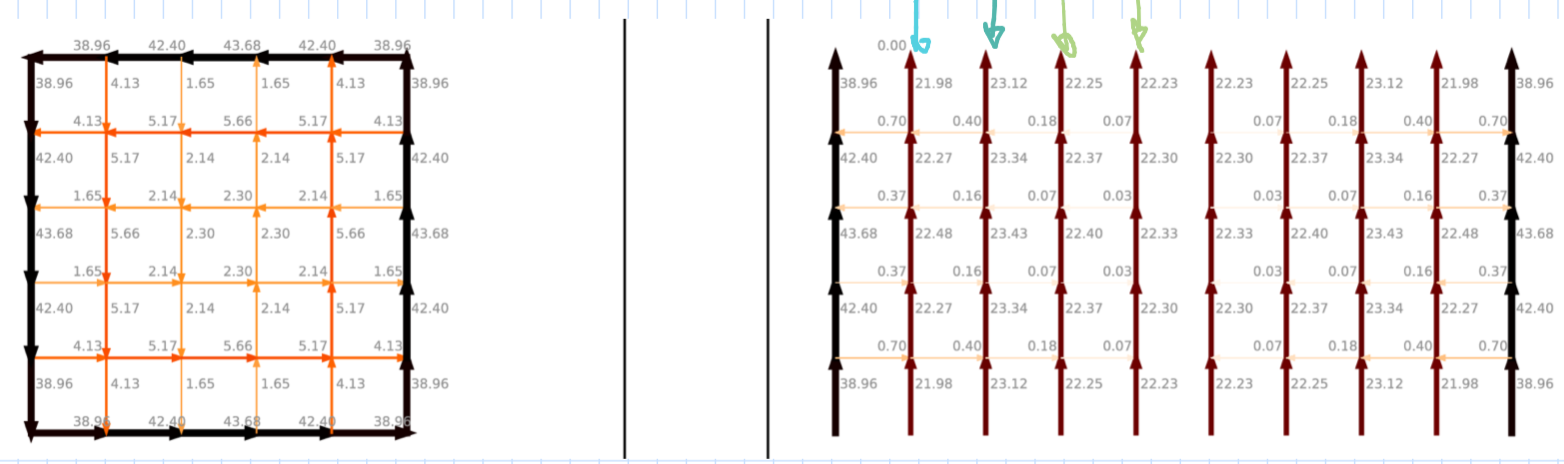
\includegraphics[width=0.9\linewidth]{gfx/prototype/coil_y_currents.png}
  \caption{The optimal current net for the $y$-coil of the ETH active magnetic field compensation system. Both $5 \times 5$ faces ($y = \mathrm{const}$ planes) are identical and are depicted on the left-hand side. The rectangular faces are identical, too, and are depicted on the right-hand side. For each segment the current per \SI{100}{\micro\tesla} of generated field is indicated upwards and to the right. CHECK}
  \label{fig:prototype_coil_y_currents}
\end{figure}

In its first version the system featured three coils for the homogeneous components of the magnetic field. The coils were designed following the method described in Ch.\,\ref{ch:coil_design} (excluding the simplification algorithm, as explained later). The fiducial volume was chosen to be a cuboid, centred in the system, \ldots away from the walls. The optimal current net for the $y$-coil is depicted in Fig.\,\ref{fig:prototype_coil_y_currents}. At the time when the system was constructed the simplification algorithm, as described in Ch.\,\ref{ch:coil_design} had not been developed, yet.

\begin{figure}
  \centering
  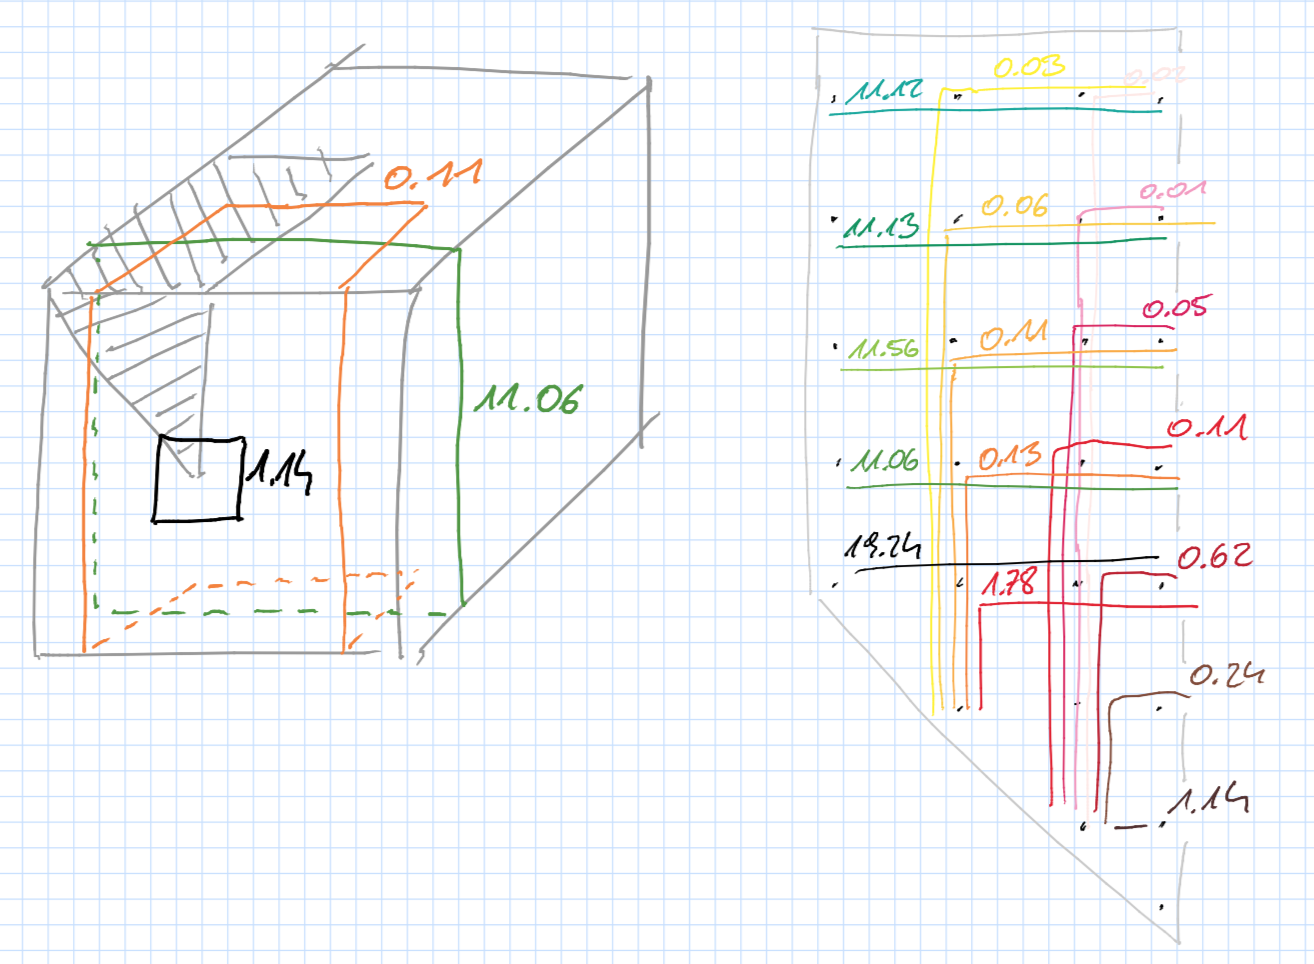
\includegraphics[width=0.4\linewidth]{gfx/prototype/coil_y_decomposition.png}
  \caption{Mention, that it shows\ldots}
  \label{fig:prototype_coil_y_decomposition}
\end{figure}

From the symmetry the $x$ and $z$ coils are identical.

\begin{figure}
  \centering
  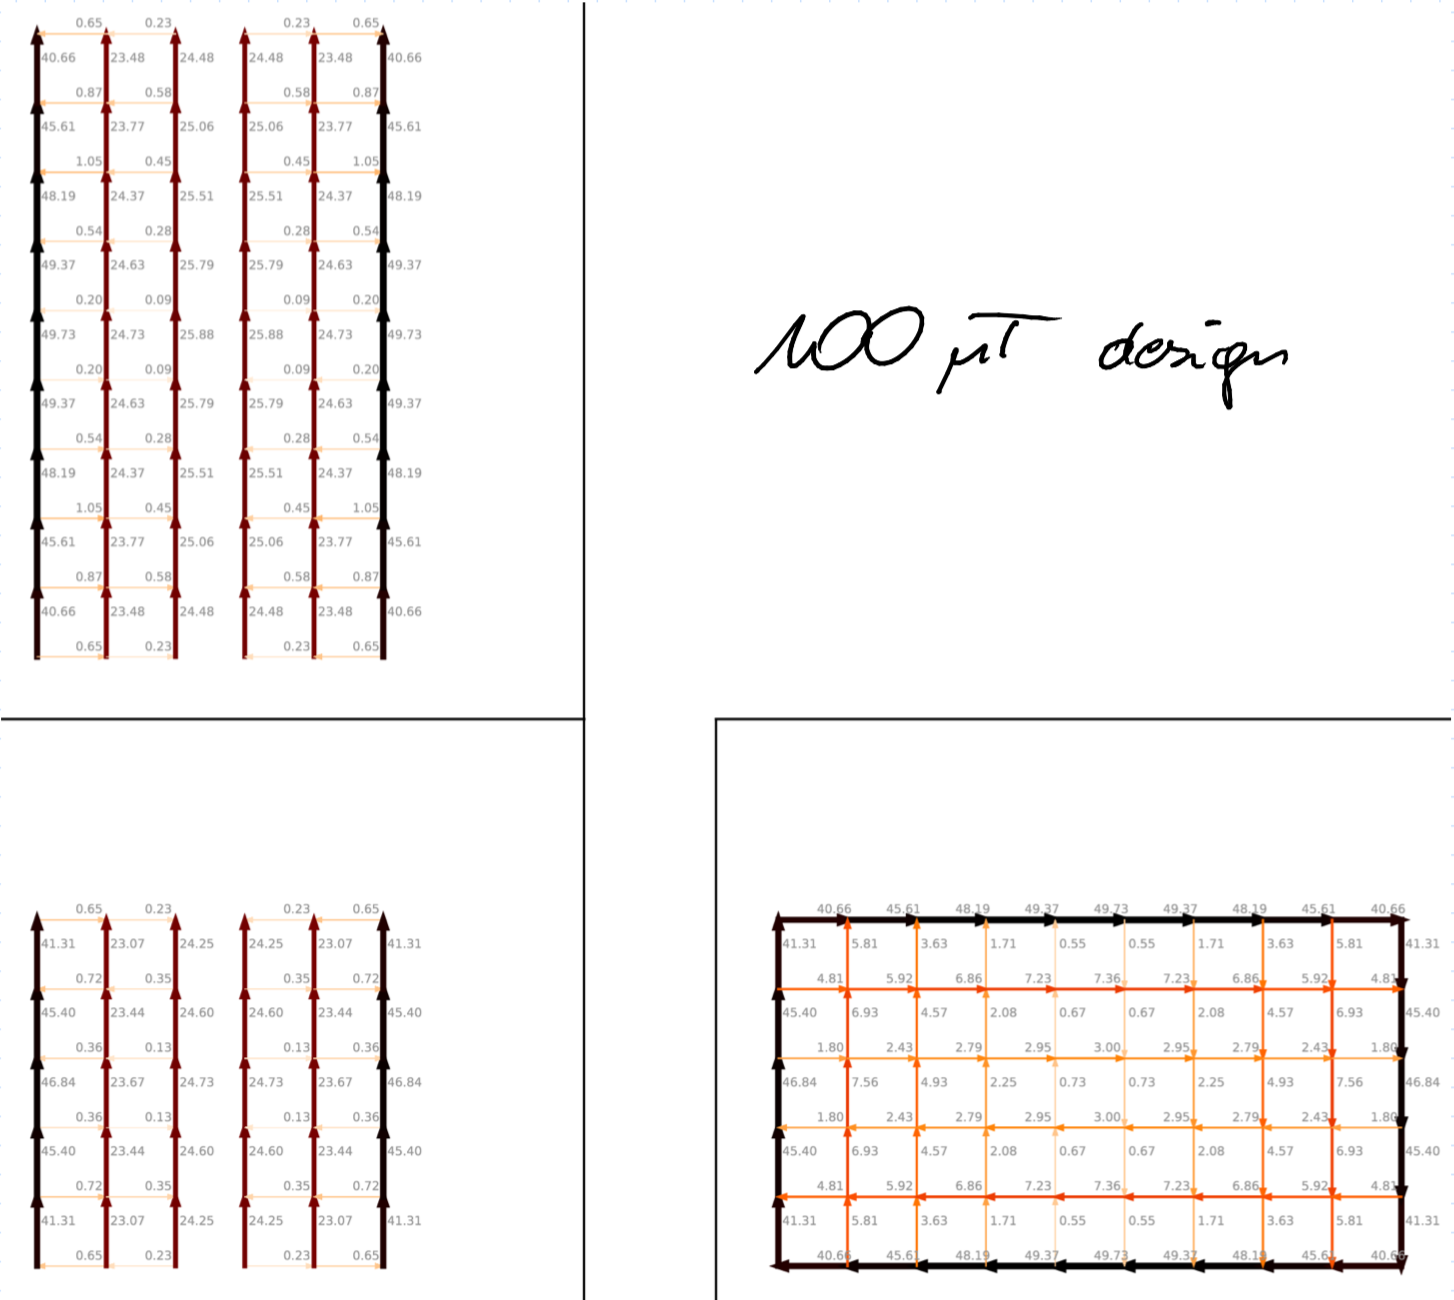
\includegraphics[width=0.9\linewidth]{gfx/prototype/coil_x_z_currents.png}
  \caption{Mention, that it shows\ldots}
  \label{fig:prototype_coil_x_z_currents}
\end{figure}

up to the point of the simplification algorithm. Here, The decomposition into loops was done by exploiting symmetries of the system. It is suboptimal in the sense, that there are more windings than there could be.

Then describe how the coils were designed. The optimized current net is shown in Fig\,\ref{fig:prototype_coil_y_currents} (for the y-coil) and \ref{fig:prototype_coil_x_z_currents} (the x- and z-coils).

It follows the already described coil design method, up to the point of the simplification algorithm. Here, The decomposition into loops was done by exploiting symmetries of the system. It is suboptimal in the sense, that there are more windings than there could be. The decompositions are depicted in Figs.\,\ref{fig:prototype_coil_y_decomposition} (the y-coil) and \ref{fig:prototype_coil_x_z_decomposition} (the x- and z-coils).



\begin{figure}
  \centering
  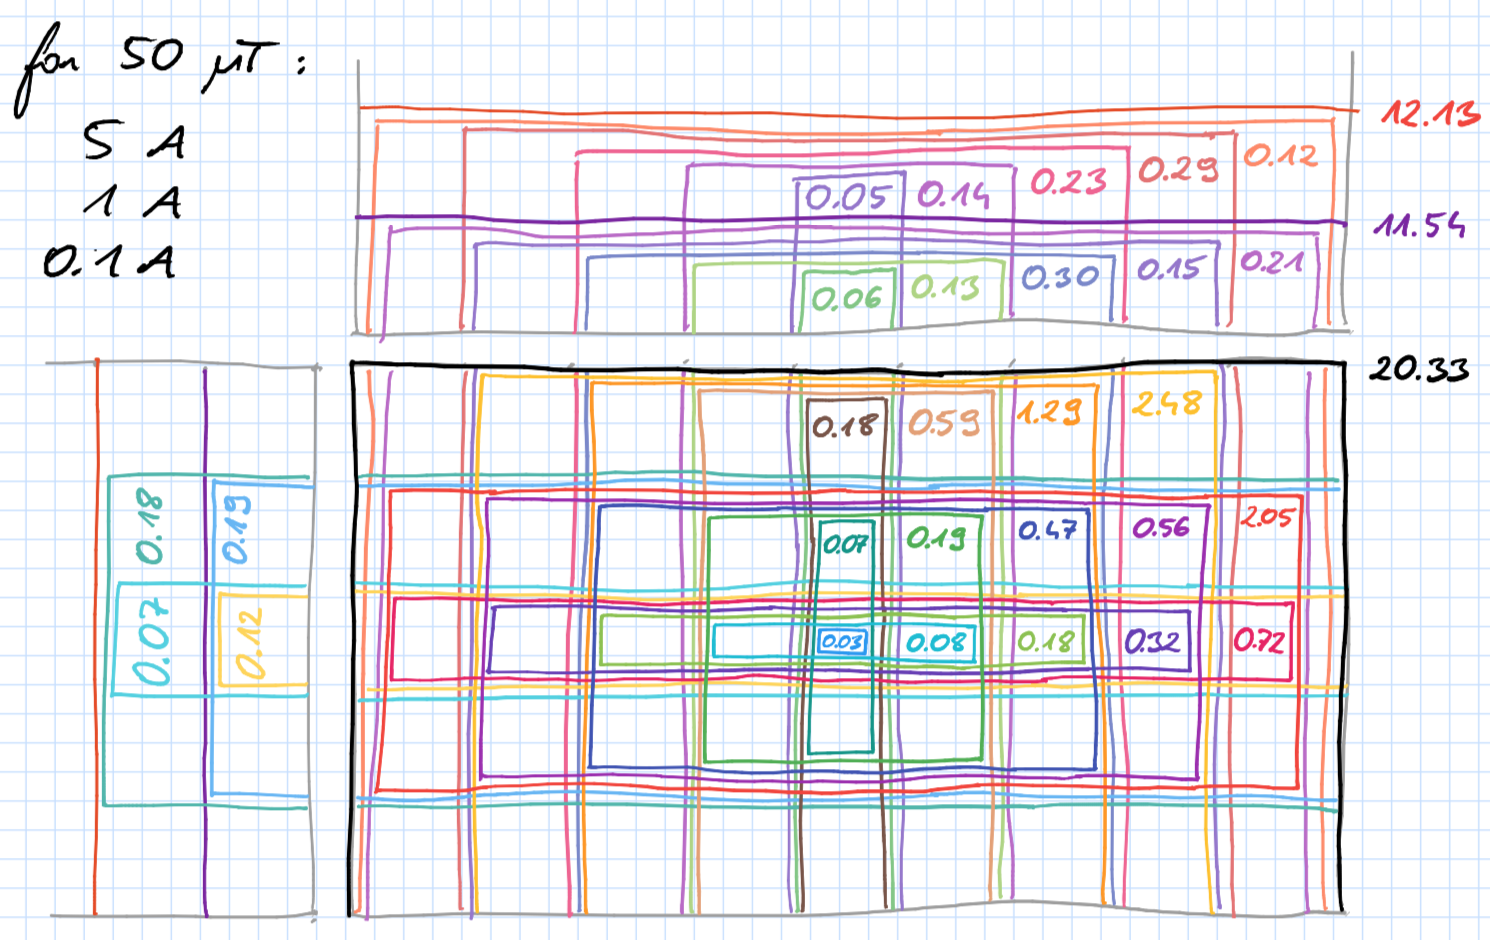
\includegraphics[width=0.9\linewidth]{gfx/prototype/coil_x_z_decomposition.png}
  \caption{Mention, that it shows\ldots}
  \label{fig:prototype_coil_x_z_decomposition}
\end{figure}

Explain how they were decomposed into the three ,,sub-coils''. Explain the nominal \SI{50}{\micro\tesla} field of each coil.



\section{Mapping}

To verify that the coils indeed produce a field of required homogeneity they were mapped. For that purpose a robot has been built---a fluxgate on an xyz-table, controlled with stepper motors.

The first map, of the y-coil, was done by moving the fluxgate along the y direction. First only the first subcoil was on, then two and finally all three. Each time they were set for the nominal \SI{50}{\micro\tesla} field. The background field was also measured and subtracted. The result is in Fig\,\ref{fig:prototype_linear_map}. Comment on the result? The field is in $\SI{\pm0.2}{\micro\tesla}$ range around the average value.

\begin{figure}
  \centering
  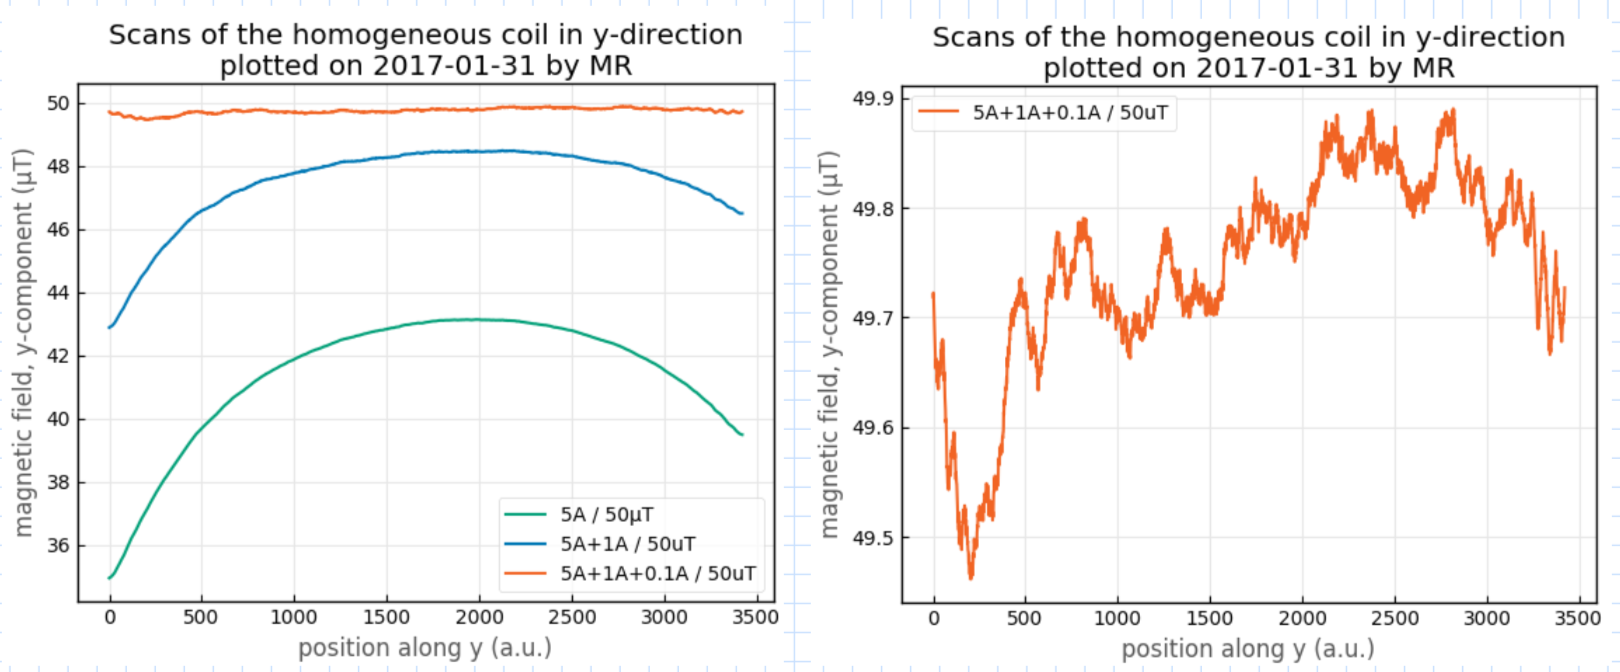
\includegraphics[width=0.9\linewidth]{gfx/prototype/linear_map.png}
  \caption{Mention, that it shows\ldots}
  \label{fig:prototype_linear_map}
\end{figure}

\begin{figure}
  \centering
  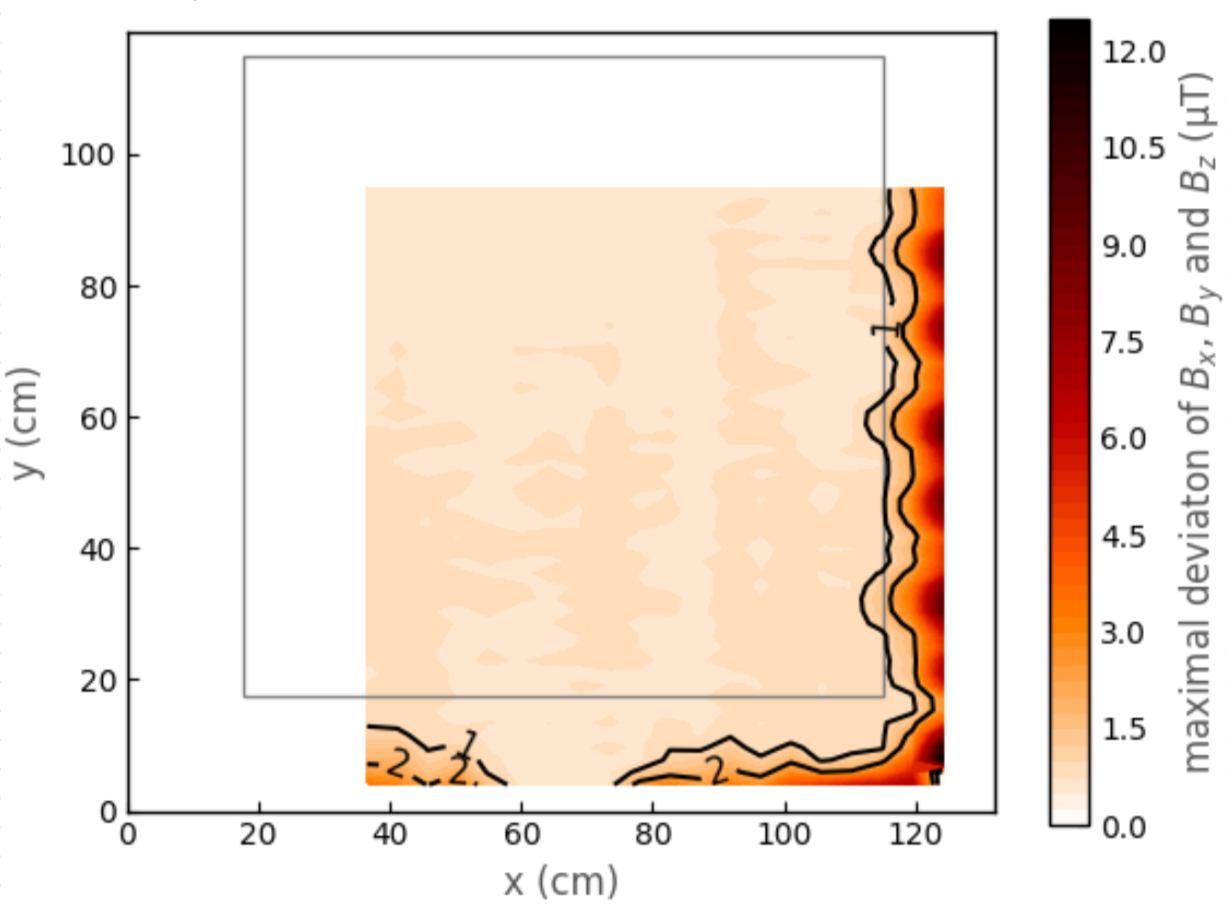
\includegraphics[width=0.9\linewidth]{gfx/prototype/plane_map.png}
  \caption{Mention, that it shows\ldots}
  \label{fig:prototype_plane_map}
\end{figure}

Now about the mapper. The device. A bar along the x direction with two timing belts fixed to it, wound around pulleys with stepper motors. The bar can slide along the y direction. Along the beam a cart can be moved in the same way with one stepper motor. On the cart three rods are mounted and a stepper motor with a threaded rod on its axis. A table can move along the three rods, with a threaded hole, when the threaded rod spins. (write in the past tense!)

\begin{figure}
  \centering
  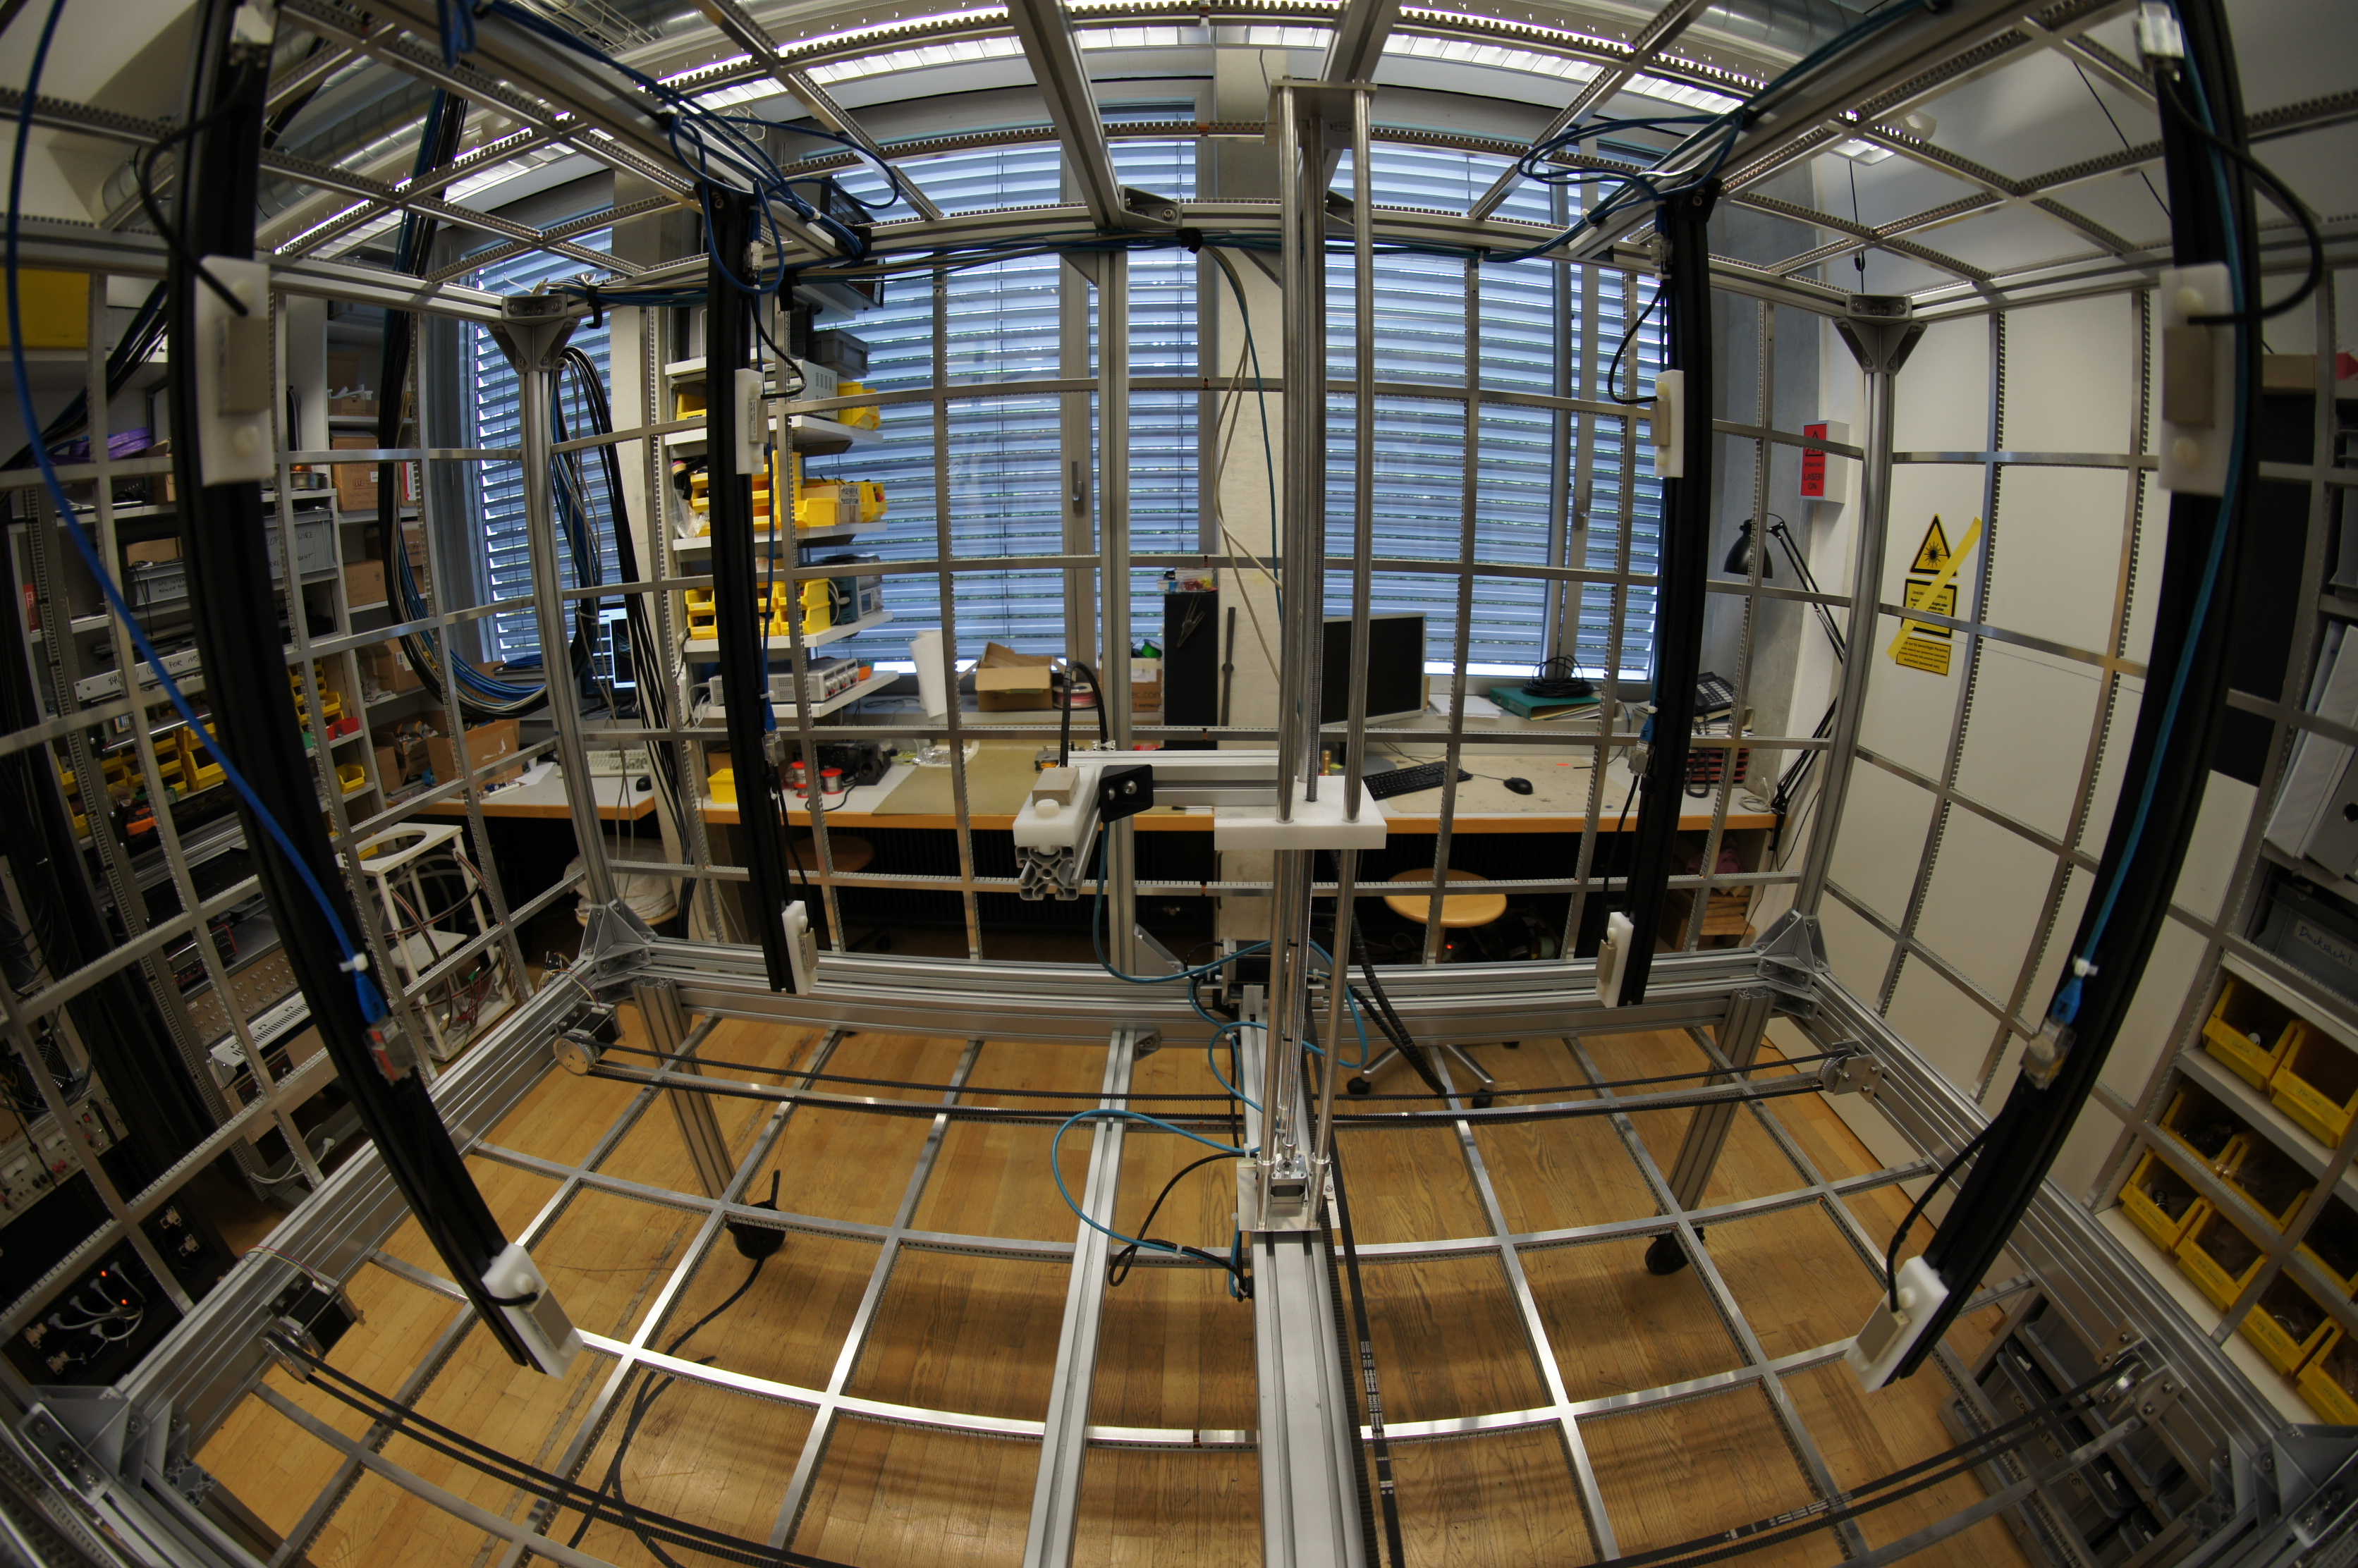
\includegraphics[width=0.9\linewidth]{gfx/prototype/DSC03476.JPG}
  \caption{Mention, that it shows\ldots}
  \label{fig:prototype_photo_inside}
\end{figure}


\section{DAQ}

\begin{figure}
  \centering
  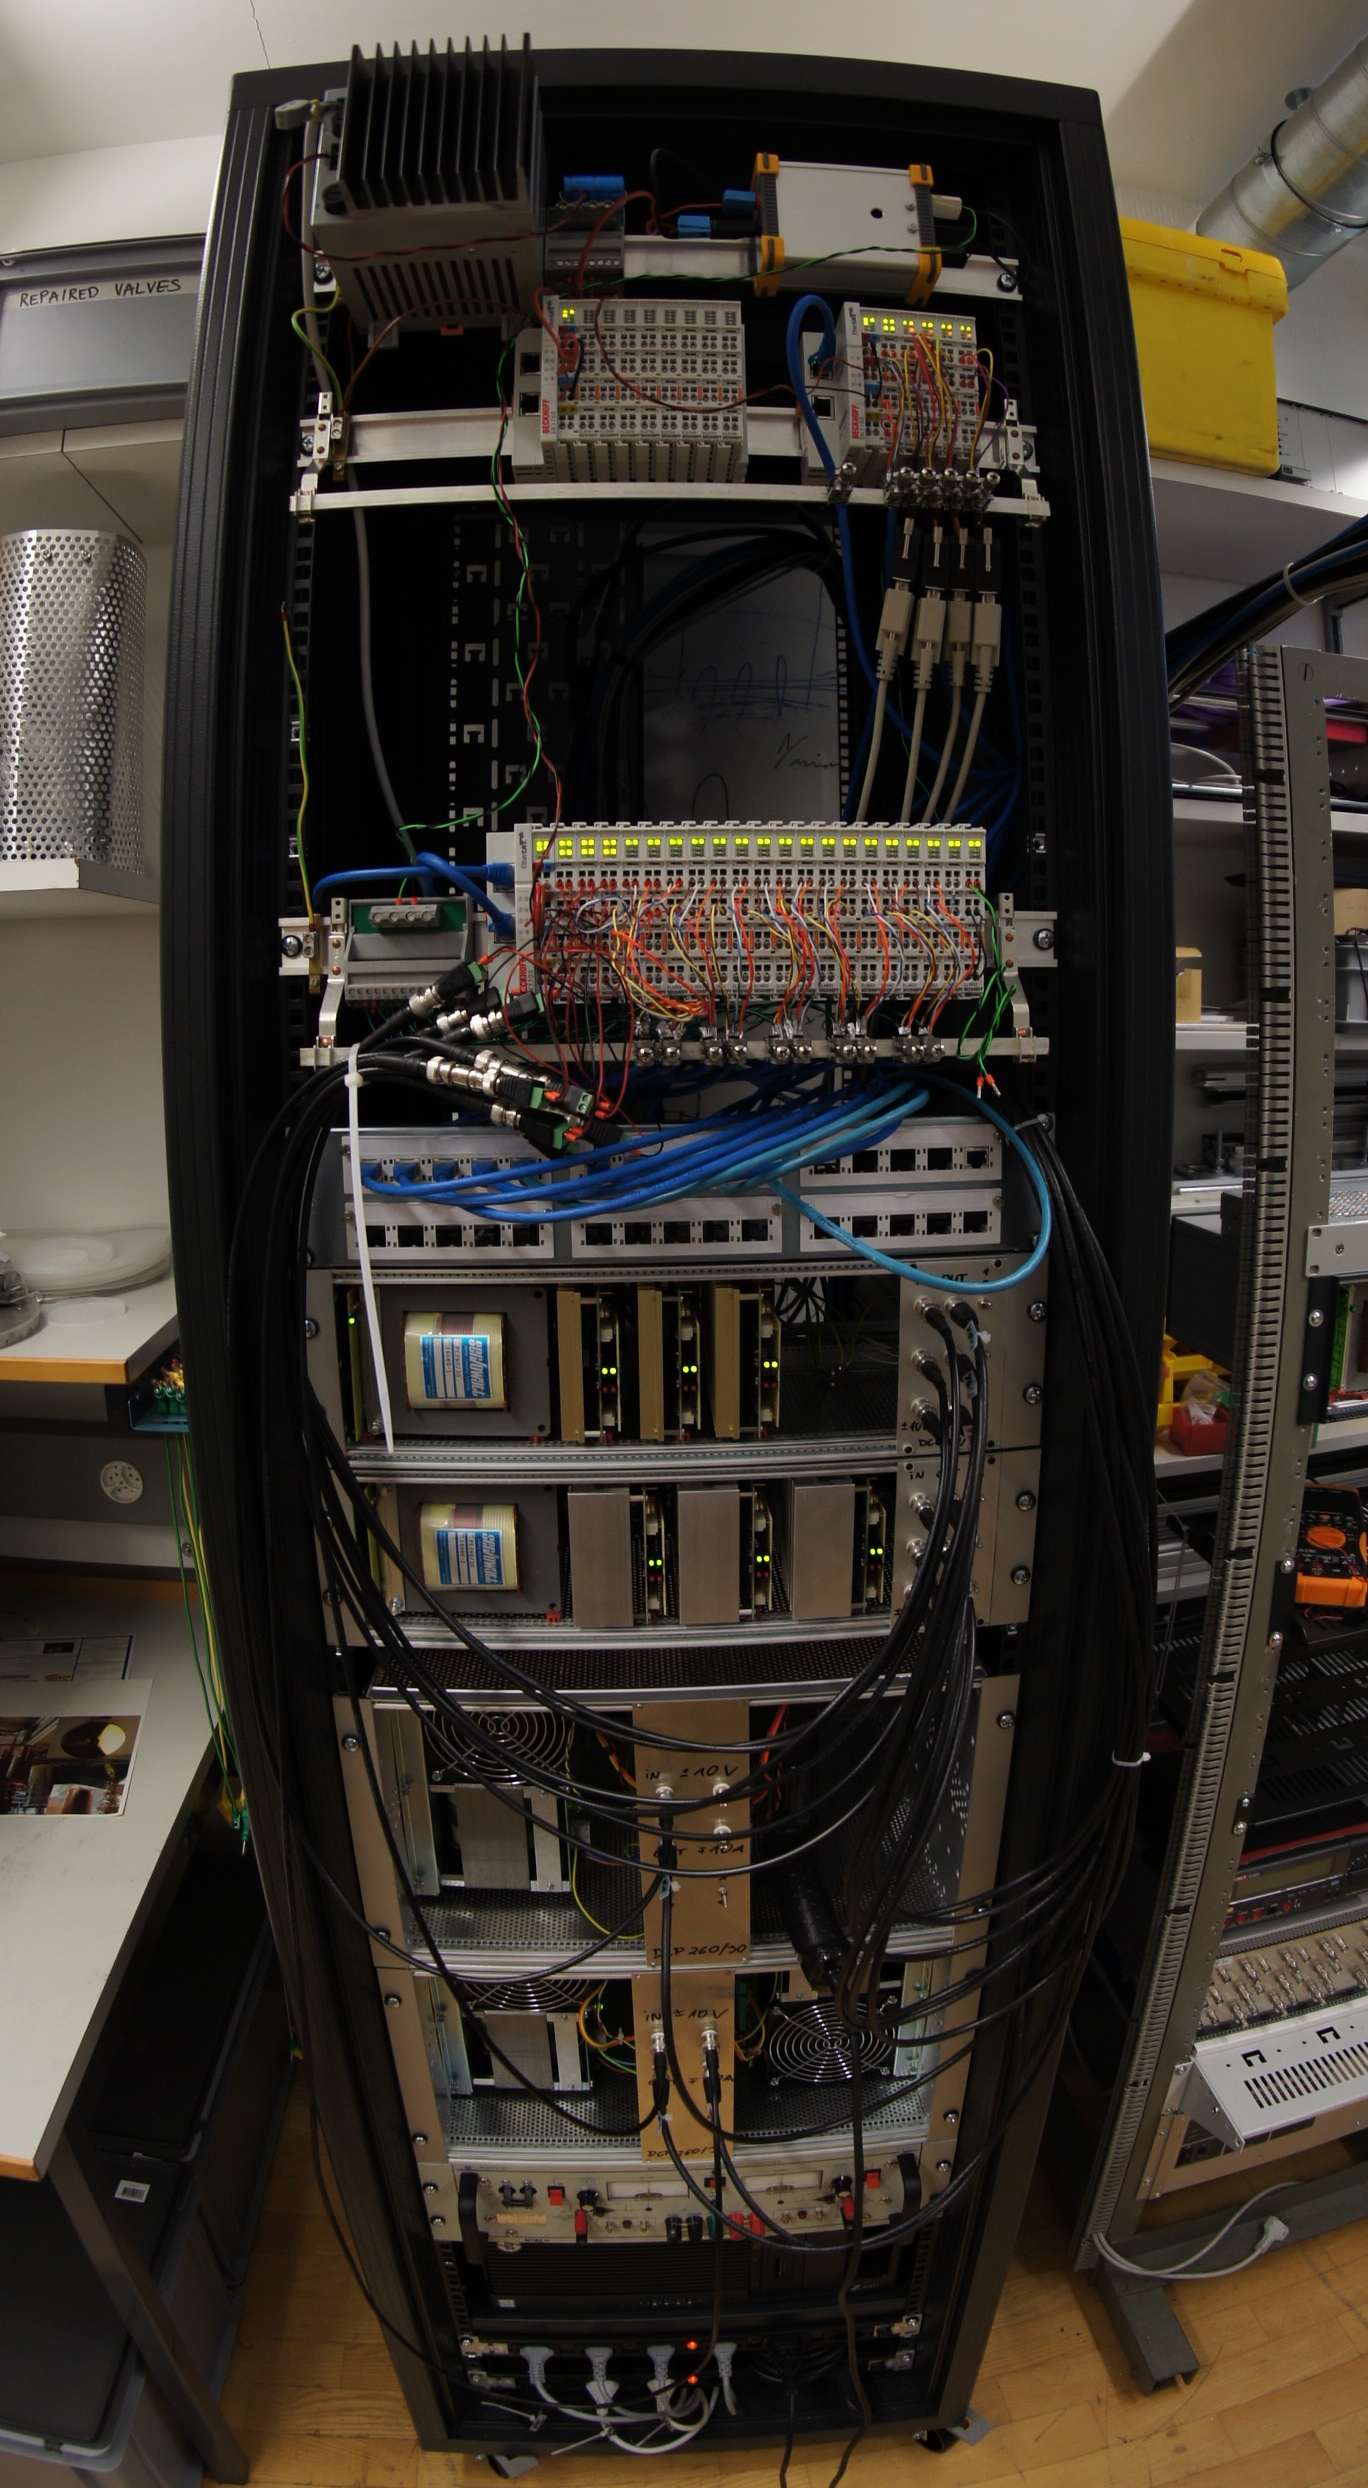
\includegraphics[width=0.6\linewidth,angle=90]{gfx/prototype/DSC03477.JPG}
  \caption{Mention, that it shows\ldots}
  \label{fig:prototype_photo_daq}
\end{figure}


Here write about the DAQ stack. Software in julia, ethercat, amplifiers, fluxgates.


\section{The SFC matrix}
Here describe the procedure of measuring the matrix, as well as the matrix itself.

Describe how the matrix is inverted to measure near the zero-field! Describe traversing the sphere and how it get smaller and smaller.

Then continue to analyse the matrix. Discuss the SVD decomposition and its singular values. Or is it the right place to do it here?


\section{The feedback algorithm}
Say, that implemented in software (julia). Write down the equation.


\section{Dynamic stabilisation}

Then show the dynamic stabilisation plot. A large permanent magnetic dipole was constructed (two neodymium magnets connected with an iron rod). It was moved

\begin{figure}
  \centering
  \subfloat{
    \label{fig:prototype_compensation_time_1}
    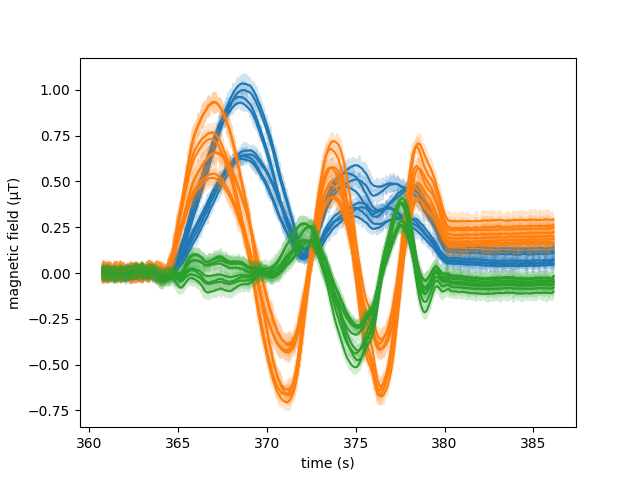
\includegraphics[width=.45\linewidth]{gfx/prototype/uncompensated_7_5m.png}}
  \quad
  \subfloat{
    \label{fig:prototype_compensation_time_2}
    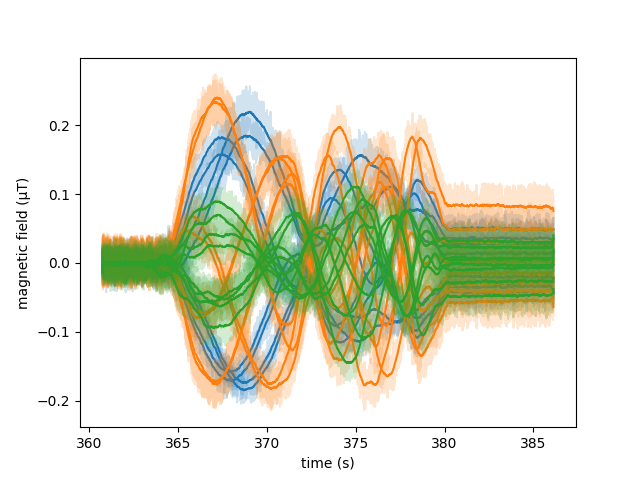
\includegraphics[width=.45\linewidth]{gfx/prototype/compensated_7_5m.png}}
  \caption{Following the algorithm to simplify a coil. The left column shows the net of a current with the total current along edges of tiles. In each iteration the loop with the highest current is found and transferred onto the simplified solution, shown in the right column. We show iterations, from top: zeroth, fourth and eighth.}
  \label{fig:prototype_compensation_time}
\end{figure}


\begin{figure}
  \centering
  \subfloat{
    \label{fig:prototype_compensation_performance}
    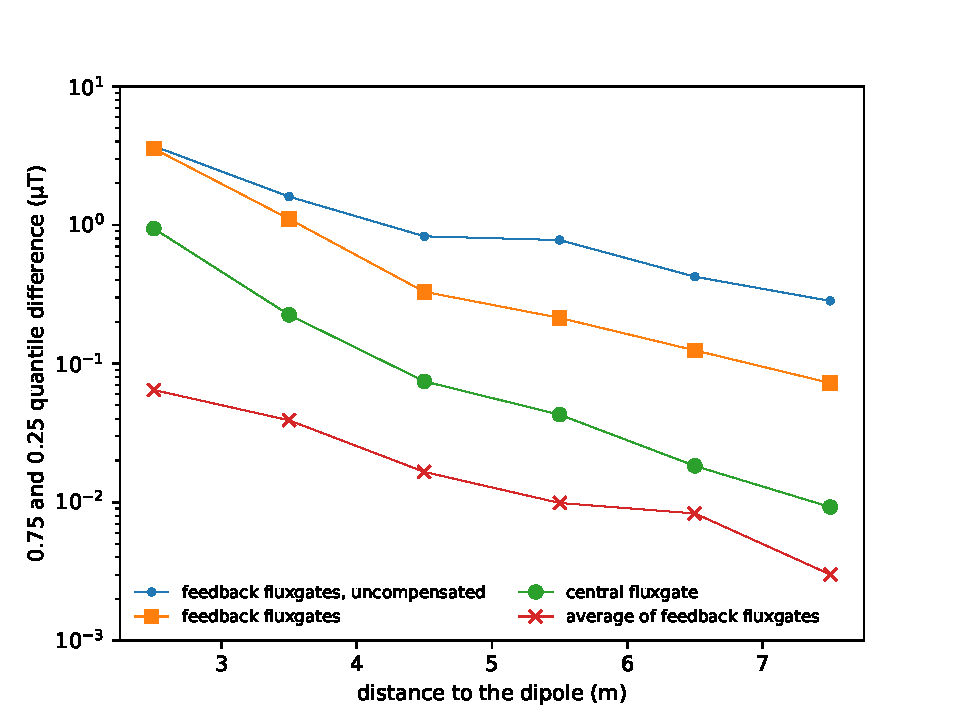
\includegraphics[width=.45\linewidth]{gfx/prototype/big_magnet_performance.pdf}}
  \quad
  \subfloat{
    \label{fig:prototype_shielding_factor}
    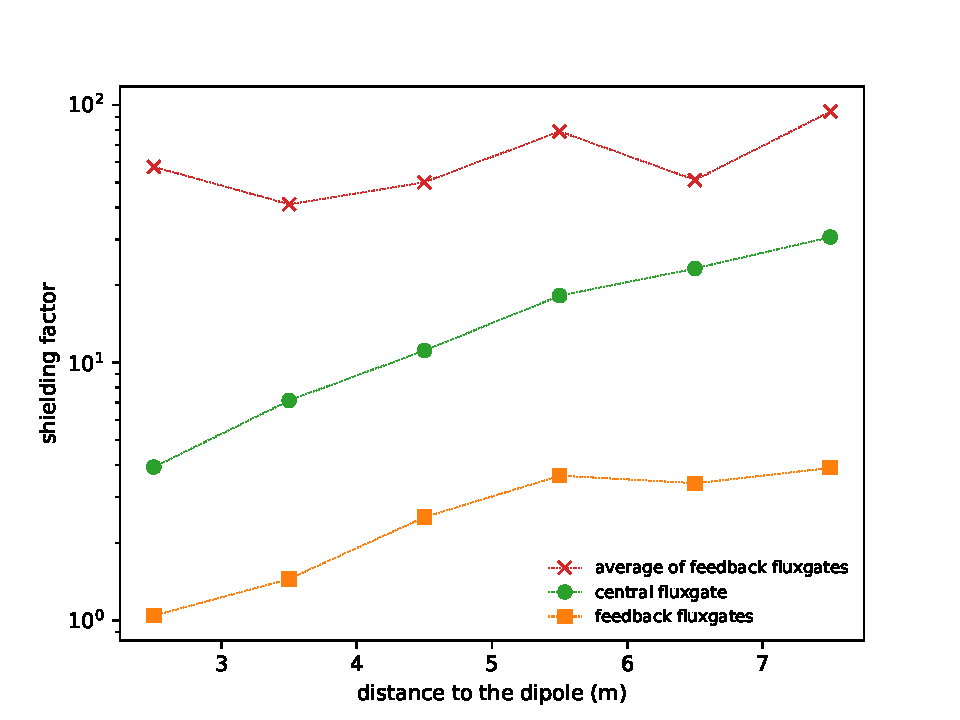
\includegraphics[width=.45\linewidth]{gfx/prototype/big_magnet_shielding_factor.pdf}}
  \caption{Following the algorithm to simplify a coil. The left column shows the net of a current with the total current along edges of tiles. In each iteration the loop with the highest current is found and transferred onto the simplified solution, shown in the right column. We show iterations, from top: zeroth, fourth and eighth.}
  \label{fig:prototype_compensation}
\end{figure}


\section{Long-term Stability}
Write about the stability. Put the stability plot. State, that it does not require the output to be stable -- the stability is defined by the stability of the input. Say, that the level of stability reached with the system corresponds to the fluxgates' specified at 0.1K temperature drift - cannot be expected to be better than that in the laboratory.

\begin{figure}
  \centering
  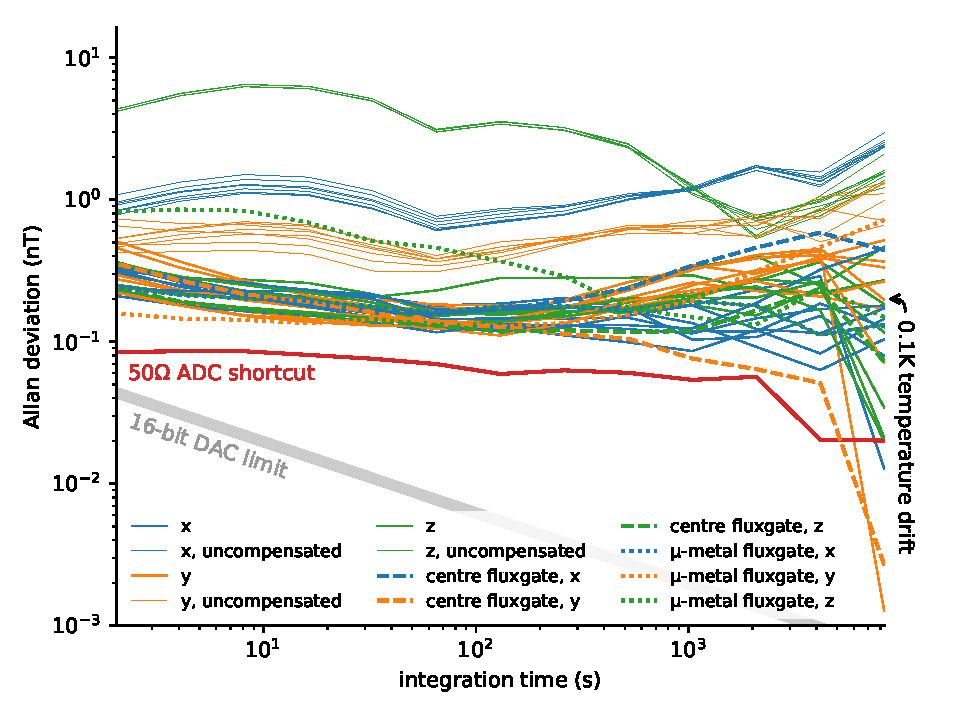
\includegraphics[width=0.9\linewidth]{gfx/prototype/run7_field_stability.pdf}
  \caption{Mention, that it shows\ldots}
  \label{fig:prototype_stability}
\end{figure}



\section{Open-design cage}

